\subsubsection{Relay Cluster Deployment}

Typical Databus deployments consist of a cluster of relay servers that pull change streams from multiple data sources. Each relay server can connect to multiple data source servers and host the change stream from each server in separate buffers in the same relay. The relays are also set up in such a way that the change stream from every data source is available in multiple relays, for fault-tolerance and for consumer scaling. There are two configurations the relays are typically deployed.

\begin{figure}
\centering
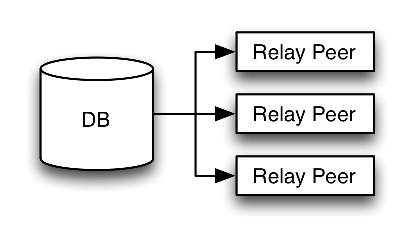
\epsfig{file=figures/relay_deployment_peers.eps, width=2.5in}
\caption{Independent Relay Deployment}
\label{fig:RelayDeployment1}
\end{figure}

In one deployment model as shown in Figure~\ref{fig:RelayDeployment1}, all the relay servers hosting a stream connect to the stream's data source directly. Each relay server is assigned a subset of all the streams being hosted by the relay cluster. The relay connects to the specified data source server and pulls the change streams. When a relay fails, the surviving relays continue pulling the change streams independent of the failed relay. If the configured redundancy factor is R, this model provides 100\% availability of the streams at very low latency as long as all the R relays that connect to the same data source server do not fail at the same time. This however comes as the cost of increased load on the data source server since there are R relays that pull the same change stream.

\begin{figure}
\centering
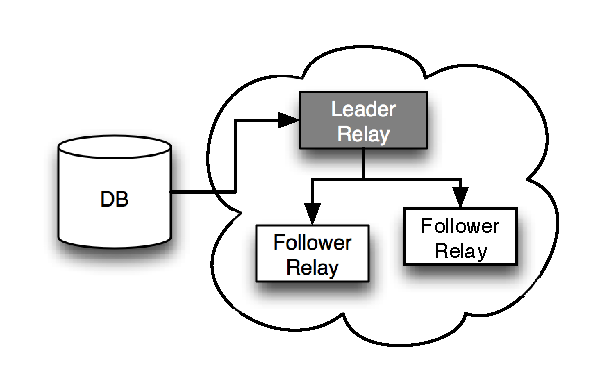
\epsfig{file=figures/relay_deployment_leader.eps, width=3in}
\caption{Leader-Follower Relay Deployment}
\label{fig:RelayDeployment2}
\end{figure}

To reduce the load on the source data source server, an alternative deployment model for relays as shown in Figure~\ref{fig:RelayDeployment2}, is the Leader-Follower model. In this model, for every data source server, one relay is designated to be the leader while R-1 are designated to be followers. The leader relay connects to the data source to pull the change stream while the follower relays pull the change stream from the leader. The clients can connect to any of the relays, either leader or follower. If the leader relay fails, one of the surviving followers is elected to be the new leader. The new leader connects to the data source server and continues pulling the change stream from the last sequence number it has. The followers disconnect from the failed leader and connect to the new leader. This deployment drastically reduces the load on the data source server but when the leader fails, there is a small delay while a new leader is elected. During this window, the latest changes in the change stream from the data source server are not available to the consumers.

To expand the capacity of the relay cluster, new relay servers can be added. When this happens, a new assignment of data source servers to relay servers is generated so that some streams are transferred from the old relay servers to the new relay servers. The new relay servers then connect to the data source servers and start pulling the change streams. They can optionally copy the existing change streams from the old relay servers before connecting to the data source servers.
This management of the relay cluster is built on top of a generic cluster management framework built at LinkedIn called Helix.

The assignment of data sources to relays is made available to Databus consumers in the form of a routing table so that the clients can discover the location of the streams they wish to consume. When the assignment changes due to relay failures or relay cluster rebalancing, this routing table is automatically updated and the consumers switch to the new servers transparently.

